% Created 2019-07-31 mi. 14:55
% Intended LaTeX compiler: pdflatex
\documentclass[a4paper,12pt,oneside]{book}
\usepackage[main=spanish, english, ]{babel}%paquete para el idioma del documento. Si
%se quiere utilizar un parrafo con idioma diferente podemos utilizar
%la orden  electlanguage{}
\usepackage[utf8]{inputenx}
\usepackage[T1]{fontenc}
\usepackage{lmodern,pifont}
\usepackage{pdflscape}
\usepackage{caption}
\usepackage{textcomp}
\usepackage{graphicx}
\usepackage{grffile}
\usepackage{wrapfig}
\usepackage{capt-of}
\usepackage[normalem]{ulem} 
\usepackage[dvipsnames]{color}
\usepackage{colortbl}
\usepackage{longtable}
\usepackage{hyperref}
\hypersetup{bookmarksopen,bookmarksnumbered,bookmarksopenlevel=4,%
  linktocpage,colorlinks,urlcolor=black,citecolor=ForestGreen,linkcolor=black,filecolor=black}
\usepackage{natbib}
\usepackage{amssymb}
\usepackage{amsmath}
\usepackage{geometry}
\geometry{a4paper,left=2cm,top=2cm,right=2.5cm,bottom=2cm,marginparsep=7pt, marginparwidth=.6in}


\newcommand{\recuerda}[1]{\begin{center}\fbox{\parbox{0.75\textwidth}{\textbf{Recuerda:}#1}}\end{center}}
\date{}
\title{MF 1481\(_{\text{2}}\). Producción de semillas}
\hypersetup{
 pdfauthor={Antonio Soler Gelde. IT Forestal},
 pdftitle={MF 1481\(_{\text{2}}\). Producción de semillas},
 pdfkeywords={},
 pdfsubject={},
 pdfcreator={Antonio Soler Gelde}, 
 pdflang={Spanish}}
\begin{document}

\maketitle
\thispagestyle{empty} \tableofcontents \clearpage\chapter{Recolección de frutos y semillas}
\label{sec:orge2e2c4b}
\section{Características de frutos y semillas}
\label{sec:orgc24742b}
El \textbf{fruto} es la parte de los vegetales que \textbf{protege la semilla} y \textbf{asegura y
dispersión}. Estrictamente el fruto es el ovario de la flor \uline{transformado y
maduro} despues de la fecundación.

En \uline{condiciones naturales, el fruto suele formarse una vez que ha tenido lugar 
la fecundación del óvulo}, pero en muchas plantas, casi siempre variedades
cultivadas, como los cítricos sin semilla, la uva, el banano y el pepino, el
fruto madura sin necesidad de fecundación; este fenómeno se llama \textbf{partenocarpia}. 

\subsection{Partes de los frutos}
\label{sec:orgb234e71}
\begin{figure}[htbp]
\centering
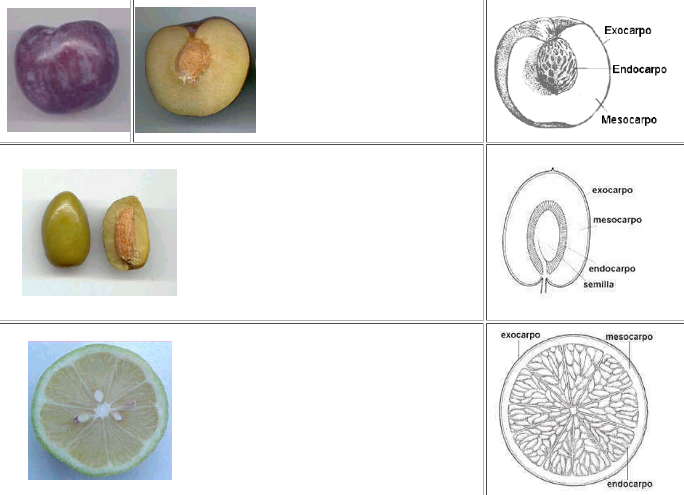
\includegraphics[width=0.8\textwidth]{./img_1481/fruto_partes_varios.PNG}
\caption{Partes de un fruto carnoso}
\end{figure}

\begin{enumerate}
\item \textbf{Epicarpio o exocarpio:} Es la capa externa que rodea al frut, corresponde
a la cáscara. Puede ser:
\begin{itemize}
\item Liso (Manzana)
\item Piloso (Melocoton)
\item Granuloso (citricos)
\item Ceroso (uva)
\end{itemize}
\item \textbf{Mesocarpio:} Es la capa intermedia y comestible del fruto. En algunos frutos
es delgado (frutos secos) y en otros carnosos
\item \textbf{Endocarpio:} Es la capa interna que envuelve a la semilla. Algunas veces es
membranosa y otras se endurece o lignifica.
\end{enumerate}

\recuerda{La semilla se encuentra encerrada \textbf{dentro del endocarpo}}
\section{Tipos de frutos}
\label{sec:orgab70174}

Existen \uline{diferentes maneras de clasificación}:

\begin{itemize}
\item Según composición y consistencia:
\begin{itemize}
\item Frutos carnosos
\item Frutos secos
\end{itemize}
\item Según número de semillas:
\begin{itemize}
\item Monospermos
\item Polispermos
\end{itemize}
\item Según forma de liberar las semillas:
\begin{itemize}
\item Dehiscentes
\item Indehiscentes
\end{itemize}
\item Según el origen del fruto
\begin{itemize}
\item Monocarpicos (Un solo carpelo)
\begin{itemize}
\item Drupa (melocotón, almendra, oliva, etc)
\item Aquenio (avellana)
\item Nucula (nuez, pistacho)
\end{itemize}
\item Policarpicos (dos o varios carpelos)
\begin{itemize}
\item Pomo (pera, manzana)
\item Baya (uva, plátano)
\item Hesperidio (naranja, mandarina, limón)
\item Balausta (granada)
\item Pepónide (papaya)
\end{itemize}
\item Multiples
\begin{itemize}
\item Polidrupa (frambuesa, mora de la zarzamora)
\item Poliaquenio (fresa)
\end{itemize}
\item Infrutescencias
\begin{itemize}
\item Sicono (higo)
\item Sorosis (chirimoya, piña, mora de la morera)
\item Cúpula (``erizo'' o involucro del castaño)
\end{itemize}
\end{itemize}
\end{itemize}

\begin{enumerate}
\item \textbf{Drupa}
\label{sec:org3a09ac2}

\begin{center}
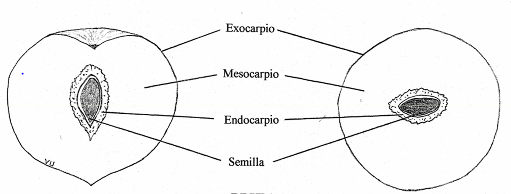
\includegraphics[width=0.8\textwidth]{./img_1481/drupa.PNG}
\end{center}

Deriva en su totalidad del ovario.

\vspace{3cm}
\item \textbf{Baya}
\label{sec:orgdc1a318}

\begin{center}
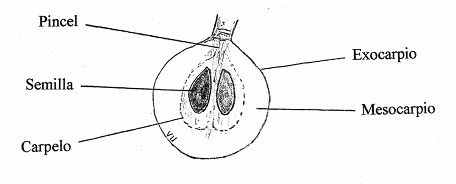
\includegraphics[width=0.8\textwidth]{./img_1481/baya.PNG}
\end{center}

\begin{itemize}
\item Deriva de un ovario simple (sin tabiques aparentes).
\item \uline{No tiene endocarpio}.
\item Es un fruto multisemillado
\end{itemize}
\newpage
\item \textbf{Pomo}
\label{sec:org351665a}

\begin{figure}[htbp]
\centering
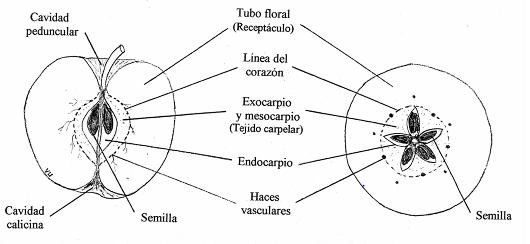
\includegraphics[width=0.8\textwidth]{./img_1481/pomo.PNG}
\caption{}
\end{figure}

Deriva de la fusión del ovario y del tubo floral (receptáculo y tejidos
adyacentes del pedúnculo). Normalmente 5 carpelos con 2 ovulos.  
\vspace{3cm}
\item \textbf{Hesperidio}
\label{sec:orga9282c8}

\begin{figure}[htbp]
\centering
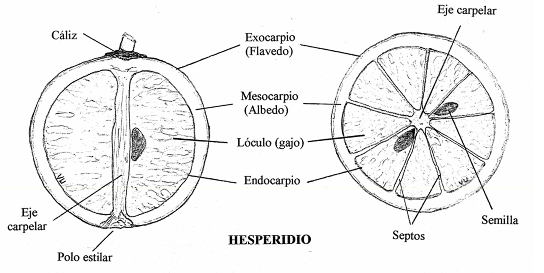
\includegraphics[width=0.8\textwidth]{./img_1481/hesperidio.PNG}
\caption{}
\end{figure}

Deriva de un ovario simple con varios carpelos. Endocarpio dividido en lóculos o
gajos.
\newpage
\item \textbf{Núcula (o nuez)}
\label{sec:org6a8bd6f}

\begin{figure}[htbp]
\centering
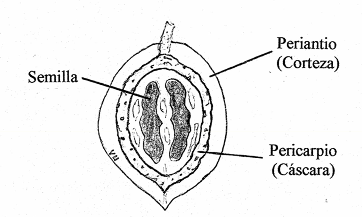
\includegraphics[width=0.8\textwidth]{./img_1481/nucula.PNG}
\caption{}
\end{figure}

\item \textbf{Agragado o múliple}
\label{sec:org0f23a78}

\begin{figure}[htbp]
\centering
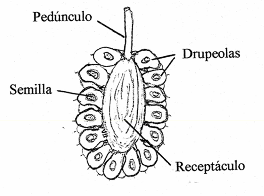
\includegraphics[width=0.8\textwidth]{./img_1481/polidrupa.PNG}
\caption{}
\end{figure}

Deriva de varios ovarios de una sola flor y de su receptáculo.

\item \textbf{Infrutescencia}
\label{sec:orgfd743f0}

\begin{figure}[htbp]
\centering
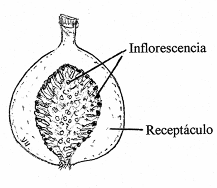
\includegraphics[width=0.8\textwidth]{./img_1481/infrutescencia.PNG}
\caption{}
\end{figure}

Deriva de launión de varios ovarios y receptaculos de una inflorescencia o
frutos simples íntimamente unidos con la apariencia de un slo fruto.
\end{enumerate}
\end{document}